\documentclass{ximera}

\begin{document}

\begin{question}
  Find 
  \[
  \displaystyle \lim_{x\to 3} f(x)
  \]
  where
  \[
  f(x) = \left\{\begin{array}{cl} x^2-x+1 & x\leq 3, \\ 2x+1 & x>3. \end{array}\right.
  \]
  \begin{solution}
    \begin{hint}
     Both $x^2-x+1$, for $x\leq3$, and $2x+1$, for $x>3$ are continuous on their respective domains. However, for the limit $\lim\limits_{x\to3}f(x)$ to exist, both the left-hand and the right-hand limits must exist and be equal.
    \end{hint}
     \begin{hint}
    	Take a look at the graph of the function
    \begin{center}
     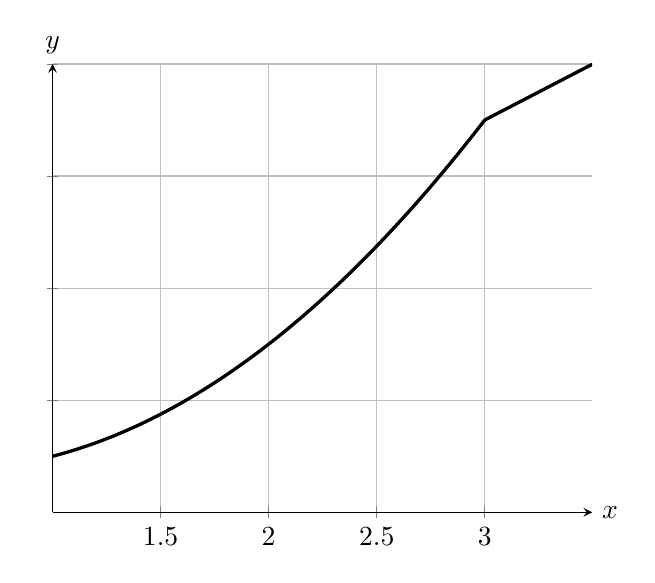
\begin{tikzpicture}
	\begin{axis}
	[ymin=0,ymax=8, axis lines=center,xlabel=$x$,ylabel=$y$,every axis y 
	label/.style={at=(current axis.above origin),anchor=south},every axis x label/.style={at=(current axis.right of origin),anchor=west},
	domain=-1:4,
	yticklabels={},
	ymajorgrids=true,
	grid = major
	]
	\addplot[domain=1:5,very thick,smooth,samples=600]
	{(!(\x>3))*(\x^2-\x+1)+(\x>3)*(2*\x+1)};
	\end{axis}
       \end{tikzpicture}      
      \end{center} 
    \end{hint}
    \begin{hint}
     Evaluating $\lim\limits_{x\to3^{+}}f(x)$ we see that it tends to $2\cdot3+1=7$. This follows because, for $x>3$, we are on the piece of $f(x)$ given by $2x+1$ and the limit $\lim\limits_{x\to3}2x+1=7$, certainly. On the other hand, evaluating $\lim\limits_{x\to3^{-}}f(x)$ we see it tends to $9-3+1=7$. This follows because, for $x\leq3$, we are on the piece of $f(x)$ given by $x^2-x+1$ and the limit $\lim\limits_{x\to3}x^2-x+1=7$, certainly. These are equal.
    \end{hint}
     The limit, $\lim\limits_{x\to3}f(x)=$
    \answer{$7$}.
  \end{solution}
\end{question}

\end{document}